\noindent Vyhľadávanie na webe, intranete alebo v~digitálnych knižniciach je dnes pravdepodobne najpoužívanejšia, no zároveň najmenej vyvinutá jazyková technológia. Google Vyhľadávač, ktorý vznikol v~roku 1998, sa v~súčasnosti využíva na vyhľadávanie 80~\% všetkých vyhľadávacích dopytov po celom svete. V~roku 2006 sa sloveso \emph{googlovať}/\emph{googliť} len veľmi tesne nestihlo zaradiť do prvého zväzku nového \emph{Slovníka súčasného slovenského jazyka}, čo sa jeho autorom neustále vyčítalo. Od prvej verzie Google sa dlhšiu dobu výrazne nezmenilo ani rozhranie vyhľadávania, ani zobrazovanie získaných výsledkov. V~súčasnej verzii ponúka Google opravu pravopisu nesprávne napísaných hľadaných slov a~v~roku 2009 začal vo svojich algoritmoch pracovať aj so základnou sémantickou analýzou\footnote{\url{http://www.pcworld.com/businesscenter/article/161869/google_rolls_out_semantic_search_capabilities.html}}, čo môže zvýšiť presnosť vyhľadávania analyzovaním významu požadovaných výrazov v~kontexte. Úspech spoločnosti Google poukazuje na fakt, že s~veľkým množstvom dostupných dát a~s~efektívnymi technikami na zaraďovanie týchto dát môže prevažne štatisticky založený prístup viesť k~uspokojivým výsledkom.

\begin{figure*}[htb]
  \colorrule{grey3}{\textwidth}{1.5pt}
  \center
  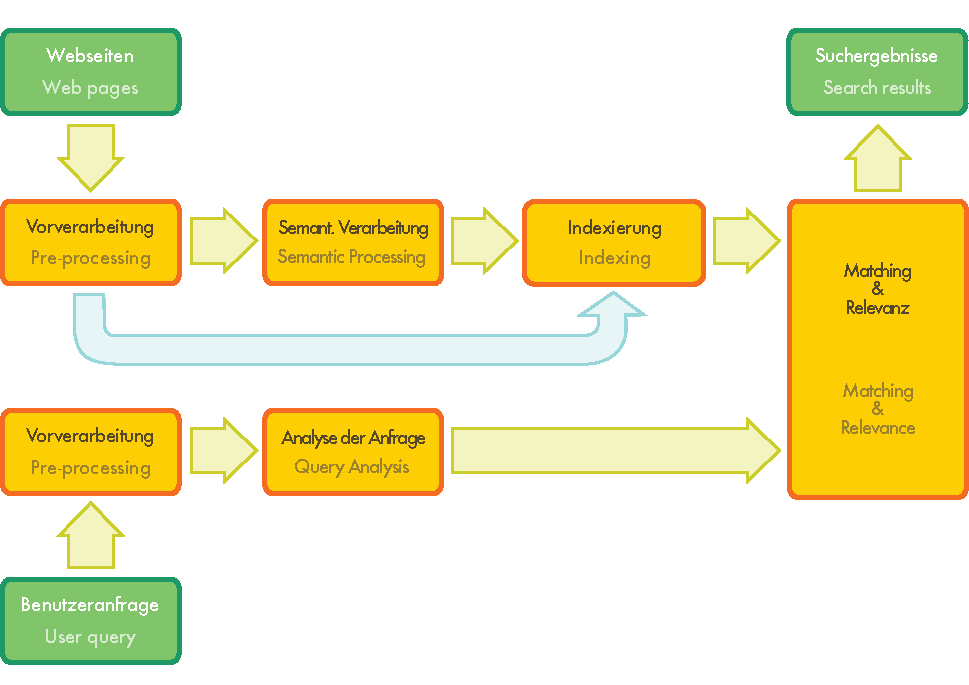
\includegraphics[width=\textwidth]{../_media/slovak/web_search_architecture}
  \caption{Architektúra vyhľadávania na webe}
  \label{fig:websearcharch_sk}
  \colorrule{grey3}{\textwidth}{1.5pt}
\end{figure*}

Pre sofistikovanejšie požadovanie informácií je však nevyhnutné integrovať hlbšie jazykové vedomosti. Experimenty vo výskumných laboratóriách s~používaním strojovo čitateľných \underbar{tezaurov} a~ontologických jazykových zdrojov ako WordNet ukázali, že je možné zvýšiť úspešnosť vyhľadávania umožnením vyhľadať stránku na základe synoným vyhľadávaných výrazov, napr. \emph{jadrová}, \emph{atómová} a~\emph{nukleárna energia} alebo dokonca aj nie veľmi súvisiacich pojmov. 

\boxtext{Budúca generácia vyhľadávačov musí zahrnúť oveľa sofistikovanejšie jazykové technológie}

Budúca generácia vyhľadávačov musí zahrnúť oveľa sofistikovanejšie jazykové technológie. Ak hľadaná požiadavka nepozostáva zo zoznamu kľúčových slov, ale z~otázky alebo z~iného typu vety, získavanie relevantnej odpovede na danú požiadavku si vyžaduje syntaktickú a~sémantickú analýzu tejto vety, ako aj dostupnosť indexu, ktorý by počítal s~rýchlym získaním relevantných dokumentov. Predstavte si napríklad zadanú vstupnú požiadavku „Dajte mi zoznam spoločností, ktoré boli za posledných\footnote{Niektorí ľudia by tu dokonca použili výraz „ostatných“ – ideálny vyhľadávací systém by si s~tým vedel poradiť.} päť rokov odkúpené inými spoločnosťami“. Pre uspokojujúcu odpoveď je potrebná syntaktická {analýza} na určenie gramatických štruktúr vety a~stanovenie faktu, že zadávateľ hľadá spoločnosti, ktoré boli odkúpené, a~nie spoločnosti, ktoré ich odkúpili. Podobne musí byť spracovaný aj výraz \emph{posledných päť rokov}, aby sa zistilo, na ktoré roky sa výraz vzťahuje. 

Pre úspešné vyhľadanie požadovanej informácie sa napokon musí spracovaná požiadavka porovnať s~obrovským množstvom neštruktúrovaných dát, v ktorých by sa vyhľadala aspoň časť požadovanej informácie. To sa často označuje termínom \underbar{získavanie informácií} a~zahŕňa vyhľadávanie a~posúdenie relevantných dokumentov. Navyše, ak chceme získať zoznam spoločností, potrebujeme extrahovať informácie, že určitý reťazec slov v~dokumente sa vzťahuje na názov spoločnosti. Tento druh informácie nám sprístupňujú takzvané \underbar{rozpoznávače pomenovaných entít}.

Ešte náročnejší je pokus spojiť zadávateľovu požiadavku
s~dokumentmi napísanými v~inom jazyku. Pre medzijazykové
získanie informácií musí byť požiadavka automaticky preložená
do všetkých možných východiskových jazykov a~získaná informácia
musí byť prenesená späť do cieľového jazyka. Rastúce percento
dát dostupných v~netextových formátoch zvyšuje dopyt po službách
umožňujúcich získavanie multimediálnych informácií,
tzn. vyhľadávanie obrázkov, zvukových a~obrazových dát. Pri
zvukových a~obrazových súboroch ide o~modul rozpoznávania
reči na konvertovanie rečového obsahu do textovej alebo fonetickej
podoby, ktorá by zodpovedala požiadavkám zadávateľa.

Na Slovensku existovali viaceré firmy, ktoré rozvíjali
technológie vyhľadávania, alebo sa takisto používali vyhľadávacie technológie
vyvinuté českými firmami. Prvý slovenský vyhľadávač, ktorý začal brať
do úvahy slovenskú morfológiu\footnote{Vyvinutý na Matematicko-fyzikálnej
fakulte Karlovej univerzity v~Prahe.}, bol \emph{morfeo.sk}, prevádzkovaný
internetovým portálom \emph{centrum.sk}, ktorý začal poskytovať fulltextové
vyhľadávanie webových stránok s~doménou \emph{.sk} v~roku 2003. Na vyhľadávanie
ohýbaných slov využíval lematizáciu a~morfologickú anotáciu, aby tak
používateľovi poskytol relevantnejšie výsledky ako len tie, ktoré zahŕňali iba
základnú formu slov. Taktiež disponoval fuzzy vyhľadávaním. Do roku 2009 presiahol počet
indexovaných stránok 117 miliónov, pretože už vtedy Google zahrnul podporu
slovenskej morfológie, prevýšil počet indexovaných stránok a~\emph{centrum.sk}
prešlo na Google Vyhľadávanie.

V~tejto oblasti pracuje napríklad Forma, s. r. o.\footnote{\url{http://www.forma.sk/}}, ktorá na báze dát z~Jazykovedného ústavu Ľ. Štúra SAV vypracovala lingvistické moduly: jazykový korektor, rozdeľovač slov, lematizátor a~slovník synoným. Takisto má samostatné produkty na fulltextové vyhľadávanie v~slovenčine a~doteraz prevádzkuje vyhľadávanie v~starších verziách niektorých slovníkov.

Pozornosť pri rozvoji vyhľadávacích technológií sa kladie na poskytovanie doplnkov a~moderných vyhľadávačov pre záujmovo špecifické portály, pričom sa čo najviac využíva sémantika relevantná pre danú oblasť. Vzhľadom na vysoké nároky na výpočtový výkon sa takéto vyhľadávače využívajú len v~relatívne malých textových korpusoch. Časom spracovania a~tisícnásobným rozsahom ľahko prekoná bežný štatistický vyhľadávač, aký poskytuje napríklad Google. Tieto vyhľadávače majú vysoké nároky aj na modelovanie tematicky zameranej domény, čo znemožňuje používať tieto mechanizmy na webe. 

Tejto oblasti výskumu sa venuje hlavne Ústav informatiky SAV, kde sa v~roku 2006 začali venovať~oblasti spracovania písaného prirodzeného jazyka. V~tom čase sa inicioval aj vznik workshopov WIKT\footnote{\url{http://conference.ui.sav.sk/wikt2010/}}, ktorých súčasťou je v~každom ročníku vydávanie niekoľkých článkov alebo celej sekcie venovanej spracovaniu slovenského jazyka. Výskum v~ÚI SAV v~spolupráci s~Univerzitou Pavla Jozefa Šafárika v~Košiciach sa od r. 2006 rozvíjal hlavne v~rámci projektu NAZOU\footnote{\url{http://nazou.fiit.stuba.sk}}, kde sa tvorili nástroje na získanie, spracovanie, organizovanie a~prezentáciu informácií z~internetu. Konkrétnou aplikáciou boli pracovné ponuky, nástroje sa testovali aj na textoch slovenských pracovných ponúk. V~ÚI SAV bola vypracovaná analýza spracovania slovenčiny \cite{laclavik2007a} a~zároveň bol vyvinutý nástroj na extrakciu informácií Ontea\footnote{\url{http://ontea.sourceforge.net/}} \cite{laclavik2007b,laclavik2009}, ktorý bol integrovaný s~nástrojmi na identifikáciu jazyka \cite{vojtek2006} a~nástrojom na lematizáciu \cite{krajci2007}.

Ontea pracuje na základe hľadania vzorov. Tieto vzory môžu byť
jednak jazykovo závislé vzory, ako napríklad použitie predložiek,
vetná skladba, ale aj jednoduchšie vzory typu použitie veľkých
písmen, skratiek, ako napríklad \emph{s. r. o.}, \emph{a. s.} na
hľadanie firiem, \emph{Sk}, \emph{SKK}, \emph{EUR}, \emph{EURO},
\emph{\euro} na hľadanie ceny, alebo skratiek slovenských krstných
mien na hľadanie osôb v~texte. Princíp je platný pre rôzne jazyky,
ale vzory sa musia tvoriť pre konkrétny jazyk, napríklad slovenčinu.
V~súčasnosti bol nástroj Ontea rozvíjaný na spracovanie e-mailovej
komunikácie. V~rámci projektu
AIIA\footnote{\url{http://aiia.ui.sav.sk/}} \cite{laclavik2010} bol
systém otestovaný na slovenských e-mailoch firmy Anasoft a~združenia
SANET. Ontea používa nielen vzory, ale aj slovníky urbanoným
(gazetteers), ako aj ich kombináciu na extrakciu a~identifikáciu
entít v~texte. Pri použití slovníkov (ale aj niektorých typov
hľadania) nastáva problém identifikácie entity, ak je v~inom ako
základnom tvare, preto~je vhodné použiť lematizátor. Keďže ide
hlavne o~názvoslovné entity ako ľudia, miesta, názvy produktov,
mená projektov alebo služieb, je ťažké ich lematizovať. Tieto
problémy sa zatiaľ nepodarilo uspokojivo vyriešiť, je však možné
riešiť ich novým spôsobom kombinácie slovníka, tokenizácie po
znakoch, lematizácie a~overenia entity v~slovníku.

Extrakcia entít pomocou vzorov bola použitá aj v~experimente na rozsiahlych dátach, keď sa spracúvali slovenské webové stránky s~cieľom extrakcie geografických dát (slovenských adries) a~následného vyhľadávania \cite{dlugolinsky2010}.
